\documentclass[10pt,letterpaper]{article}
%\usepackage{savetrees}
\usepackage[margin=1.2cm]{geometry}
\usepackage{xcolor}
\usepackage{microtype}
\usepackage{amsmath}
\usepackage{amsfonts}
\usepackage{amssymb}
\usepackage{mathtools}
\usepackage{array}
\usepackage{booktabs}
\usepackage{multirow}
\usepackage{bbm}
\usepackage{hyperref}
\usepackage{latexsym}
\usepackage{expl3}
\usepackage{tikz}
\usetikzlibrary{matrix}
\usepackage{stackengine}
\usepackage{etoolbox}
%\usepackage{mathabx}
\usepackage{graphicx}
\usepackage{enumitem}
\usepackage{etoc}

\newcommand*{\myetocenumeratesetup}{}
\protected\def\myetocenumeratesetup{%
  \setlist[enumerate]{label=\etocnumber,
    topsep=0pt,parsep=0pt,partopsep=0pt,itemsep=0pt,
    rightmargin=0pt,
    leftmargin=0pt,
    labelindent=0pt,
    labelsep=0pt,
    align=left,
  }%
  \sloppy\raggedright}
% leftmargin + itemindent = labelindent + labelwidth + labelsep

\setcounter{tocdepth}{5}
\etocmulticolstyle[2]{\myetocenumeratesetup\setlength{\columnsep}{10pt}\setlength{\columnseprule}{.4pt}}
\etocsetstyle{section}
  {\begin{enumerate}[labelwidth=14pt,leftmargin=14pt]}
  {\footnotesize\normalfont\bfseries\item}
  {\etocname{}\nobreak\hfill\etocpage}
  {\end{enumerate}}
\etocsetstyle{subsection}
  {}
  {\scriptsize\normalfont\item}
  {\etocname{} \hbox{}\nobreak\hfill\etocpage}
  {}
\etocsetstyle{subsubsection}{\ERROR}{}{}{}
\etocsetstyle{paragraph}
  {\begin{enumerate}[leftmargin=-8pt]}
  {\tiny\normalfont\item}
  {\etocname{}}
  {\end{enumerate}}
\etocsetstyle{subparagraph}{\ERROR}{}{}{}

\hypersetup{unicode}
\hypersetup{linktoc = all}                % hyperref settings
\hypersetup{hidelinks = true}
\pdfstringdefDisableCommands{%
  \def\({}%
  \def\){}%
  \def\\{}%
  \def\pi{\003\300}%
  \edef\sb{\string _}%
  \def\leq{\042\144}%
  \def\infty{\042\036}%
  \def\Tr{Tr }%
}

\setcounter{secnumdepth}{2}
\makeatletter
\renewcommand{\section}{\pagebreak[1]\@startsection {section}{1}{\z@ }{-\medskipamount}{\smallskipamount}{\normalfont \large \bfseries }}
\renewcommand{\subsection}{\pagebreak[0]\@startsection {subsection}{2}{\z@ }{-\smallskipamount}{1sp}{\normalfont \bfseries }}
\renewcommand{\subsubsection}{\ERROR}
\renewcommand{\paragraph}[1]{\@startsection {paragraph}{3}{\z@ }{-\smallskipamount}{-1sp}{\normalfont \bfseries }{#1}\hspace{0pt}}
\makeatother
%%% Sorry the next two lines are a bit horrible
%\renewcommand{\paragraph}[1]{\par\noindent\textbf{#1}}
%\newcommand{\definition}{\par\noindent\textbf{Def.} \ignorespaces}
%\newcommand{\proposition}{\par\noindent\textbf{Prop.} \ignorespaces}
\setlength{\parskip}{2pt plus 2pt minus 2pt}
\setlength{\baselineskip}{10pt}

\newcommand{\tabfoot}[1]{\leavevmode\ensuremath{{}^{\tabfootsymb{#1}}}}
\makeatletter
\newcommand{\tabfootsymb}[1]{\ensuremath{\scriptstyle\@fnsymbol{\the\numexpr(#1)+2\relax}}}
\makeatother

%%%%%%%%%%%%%%%%%%%%%%%%%%%%%%
% http://tex.stackexchange.com/questions/14386/importing-a-single-symbol-from-a-different-font
\DeclareFontFamily{U}{mathb}{\hyphenchar\font45}
\DeclareFontShape{U}{mathb}{m}{n}{
      <5> <6> <7> <8> <9> <10> gen * mathb
      <10.95> mathb10 <12> <14.4> <17.28> <20.74> <24.88> mathb12
      }{}
\DeclareSymbolFont{mathb}{U}{mathb}{m}{n}
\DeclareFontSubstitution{U}{mathb}{m}{n}
\DeclareMathSymbol{\righttoleftarrow}{3}{mathb}{"FD}
%%%%%%%%%%%%%%%%%%%%%%%%%%%%%%

%\newcommand{\defined}[1]{\textsl{#1}}
\newcommand{\actson}{\mathrel{\reflectbox{$\righttoleftarrow$}}}
\newcommand{\dd}[2][]{\mathop{\mathrm{d}\mkern0mu\relax#1#2}}%\mkern avoids \mathop{d} (vertical placement issue)
\newcommand{\ie}{i.e.\@}
\newcommand{\eg}{e.g.\@}
\newcommand{\Eg}{E.g.\@}
\makeatletter
\newcommand{\etc}{etc.\@ifnextchar.{\@gobble}{\@}}
\makeatother
\newcommand{\I}{\mathrm{i}}
\newcommand{\E}{\mathrm{e}}
\newcommand{\Wedge}{\bigwedge}
\newcommand{\del}{\partial}
\newcommand{\delbar}{\overline{\partial}}
\newcommand{\Nsusy}{{\mathcal{N}}}
\newcommand{\repr}[1]{\mathbb{#1}}
\newcommand{\todo}[1]{\emph{todo: #1}}
\newcommand{\cyclic}[1]{\ZZ_{#1}}
\newcommand{\ZZ}{\mathbb{Z}} % integers
\newcommand{\QQ}{\mathbb{Q}} % rationals
\newcommand{\RR}{\mathbb{R}} % reals
\newcommand{\CC}{\mathbb{C}} % complex
\newcommand{\HH}{\mathbb{H}} % quaternions
\newcommand{\PP}{\mathbb{P}} % projective
\newcommand{\torus}{\mathbf{T}} % torus
\DeclarePairedDelimiter{\abs}{\lvert}{\rvert}
\DeclareMathOperator{\End}{End}
\DeclareMathOperator{\Tr}{Tr}
\DeclareMathOperator{\plexp}{plexp}
\DeclareMathOperator{\rank}{rank}

\ExplSyntaxOn
\newcommand{\Lie}[1]{
  \mathrm {
    \clist_if_in:nnF
      { GL , SL , SO , SU , U , O , Sp , USp , OSp , Spin , A , B , C , D , E , F , G , P , Q , UQ , W , S , \tilde S , \tilde{S} , H }
      {#1} { \UnknownLie }
    #1
  }
}
\newcommand{\lie}[1]{
  \mathfrak {
    \str_case:nnF {#1}
      {
        { sl } { sl }
        { so } { so }
        { su } { su }
        { u } { u }
        { o } { o }
        { sp } { sp }
        { usp } { usp }
        { osp } { osp }
        { A } { a }
        { B } { b }
        { C } { c }
        { D } { d }
        { E } { e }
        { F } { f }
        { G } { g }
        { P } { p }
        { Q } { q }
        { UQ } { uq }
        { W } { w }
        { S } { s }
        { \tilde S } { \tilde s }
        { \tilde{S} } { \tilde{s} }
        { H } { h }
      } { \ERROR #1 }
  }
}
\ExplSyntaxOff
%\robustify\tilde

\newcommand{\undovskip}{\relax\ifvmode\ifdim\lastskip>0pt\relax\vskip-\lastskip\fi\fi}
\newenvironment{tab}[1]{\center\undovskip\vspace{.1\baselineskip}\tabular{#1}\toprule}{\crcr\bottomrule\endtabular\endcenter\undovskip\vspace{.1\baselineskip plus .3\baselineskip}}



\begin{document}
\twocolumn\raggedbottom

\noindent\textbf{\Large Tables for supersymmetry.}

\noindent Bruno Le Floch, Princeton University, \today.

\let\contentsname\empty
{\tiny\tableofcontents\par}\undovskip

\section{Special functions}

% todo: Euler's Gamma function, elliptic Gamma function, hyperbolic Gamma function, Barnes' double-Gamma function, multiple sine, Upsilon, Dedekind eta function, Jacobi theta functions,

\paragraph{Plethystic exponential.}  Let $\mathbf{m}\subset R[[x_1,\ldots,x_n]]$ be series with no constant term over a ring~$R$.  Then $\plexp:\mathbf{m}\to 1+\mathbf{m}$ obeys $\plexp[x_i^p]=1/(1-x_i^p)$ and $\plexp[\lambda f]=\plexp[f]^\lambda$ for $\lambda\in R$.  It maps an index of single-particle states $f(x)$ to that of multiparticle states $\plexp f(x)=\exp\sum_{k\geq 1}\frac{1}{k}f(x_1^k,\ldots,x_n^k)$.

\paragraph{Dedekind eta function.}  Modular form of weight~$\frac{1}{2}$ given by $\eta(\tau)=q^{1/24}\prod_{k\geq 1} (1-q^k)=q^{1/24}\plexp[\frac{-q}{1-q}]$ where $q=\E^{2\pi\I\tau}$.

\paragraph{Theta function.}  $\vartheta_1(x;q)=-\I x^{1/2}q^{1/8}\plexp[-\frac{q+xq+1/x}{1-q}]=-\I x^{1/2}q^{1/8}\prod_{k\geq 1} (1-q^k)(1-xq^k)(1-q^{k-1}/x)$.



\section[Lie algebras and groups]{Lie algebras and groups (dimension${}<\infty$)}

\subsection{Simple Lie (super)algebras}

\paragraph{Complex case.}
Infinite series $\lie{A}_{n\geq 1}$, $\lie{B}_{n\geq 1}$, $\lie{C}_{n\geq 1}$, $\lie{D}_{n\geq 2}$ with
$\lie{A}_1=\lie{B}_1=\lie{C}_1$, $\lie{B}_2=\lie{C}_2$, $\lie{D}_2=\lie{A}_1\oplus \lie{A}_1$, $\lie{D}_3=\lie{A}_3$.
Five exceptions with
%
dimensions
\begin{tabular}{|ccccc|}
 $\lie{E}_6$ & $\lie{E}_7$ & $\lie{E}_8$ & $\lie{F}_4$ & $\lie{G}_2$ \\
 $78$ & $133$ & $248$ & $52$ & $14$ \\[-1ex]
\end{tabular} .
% $\dim(\lie{E}_6)=78$, $\dim(\lie{E}_7)=133$, $\dim(\lie{E}_8)=248$, $\dim(\lie{F}_4)=52$, $\dim(\lie{G}_2)=14$.
\begin{tab}{*{3}{>{$}l<{$}}l}
  \text{Type} & \text{Dimension} & \text{Lie algebra} \\\midrule
  \lie{A}_n & n(n+2) & \lie{sl}(n+1,\CC) =\{\text{traceless}\} \\
  \lie{B}_n & n(2n+1) & \lie{so}(2n+1,\CC) =\{\text{antisymmetric}\} \\
  \lie{C}_n & n(2n+1) & \lie{sp}(2n,\CC)
	=\left\{\left(\begin{smallmatrix}0&\mathbbm{1}_n\\-\mathbbm{1}_n&0\end{smallmatrix}\right)\times\text{symmetric}\right\}
  \\
  \lie{D}_n & n(2n-1) & \lie{so}(2n,\CC) =\{\text{antisymmetric}\} \\
\end{tab}

\paragraph{Real case.}\hspace{0pt minus 1pt}  Let
$\lie{sl}(n)=\lie{sl}(n,\RR)$,
$\lie{su}^*(2n)=\lie{sl}(n,\HH)$,
$\lie{so}^*(2n)=\lie{o}(n,\HH)$,
$\lie{sp}(m,n)=\lie{usp}(2m,2n)=\lie{u}(m,n,\HH)$.
A Lie algebra is compact if it exponentiates to a compact Lie group.
In $\lie{E}_{r(s)}$, $s$ is the number of $(\text{non-compact})-(\text{compact})$ generators.
\begin{tab}{@{}c@{ }lll}
& Real form & \hspace{-1em}Max compact subalgebra & Range \\
\midrule
\multirow{4}{*}{\rotatebox{90}{$sl(n)$}}
& $\lie{su}(n)$ & compact & \\
& $\lie{sl}(n)$ & $\lie{so}(n)$ & \\
& $\lie{su}(n-p,p)$ & $\lie{su}(n-p)\oplus \lie{su}(p)\oplus \lie{u}(1)$ & $0<p<n$ \\
& $\lie{su}^*(n)$ & $\lie{usp}(n)$ & $n$ even \\
\midrule
\multirow{3}{*}{\rotatebox{90}{$\lie{so}(n)$}}
& $\lie{so}(n)$& compact & \\
& $\lie{so}(p,n-p)$& $\lie{so}(p)\oplus \lie{so}(n-p)$ & $0<p<n$ \\
& $\lie{so}^*(n)$   & $\lie{u}(n/2)$ & $n$ even \\
\midrule
\multirow{3}{*}{\rotatebox{90}{$\lie{sp}(2n)$}}
& $\lie{usp}(2n)$ & compact & \\
& $\lie{sp}(2n,\RR)$  & $\lie{u}(n)$ & \\
& $\lie{usp}(2n-2p,2p)$ & $\lie{usp}(2n-2p)\oplus \lie{usp}(2p)$ & $0<p<n$ \\
\midrule
\multicolumn{4}{c}{%
  \begin{tabular}[c]{ll}
  $\lie{E}_{6(-78)}$ & compact \\
  $\lie{E}_{6(-26)}$ & $\Lie{F}_4$ \\
  $\lie{E}_{6(-14)}$ & $\lie{so}(10)\oplus \lie{so}(2)$\\
  $\lie{E}_{6(2)}$ & $\lie{su}(6)\oplus \lie{su}(2)$\\
  $\lie{E}_{6(6)}$ & $\lie{usp}(8)$\\
  \midrule
  $\lie{E}_{7(-133)}$& compact \\
  $\lie{E}_{7(-25)}$& $\lie{E}_{6,-78}\oplus \lie{so}(2)$ \\
  $\lie{E}_{7(-5)}$& $\lie{so}(12)\oplus \lie{su}(2)$ \\
  $\lie{E}_{7(7)}$& $\lie{su}(8)$
  \end{tabular}\quad
  \begin{tabular}[c]{ll}
  $\lie{E}_{8(-248)}$& compact\\
  $\lie{E}_{8(-24)}$&$\lie{E}_{7,-133}\oplus \lie{su}(2)$\\
  $\lie{E}_{8(8)}$&$\lie{so}(16)$\\
  \midrule
  $\lie{G}_{2(-14)}$ & compact \\
  $\lie{G}_{2(2)}$ & $\lie{su}(2)\oplus \lie{su}(2)$ \\
  \midrule
  $\lie{F}_{4(-52)}$ & compact \\
  $\lie{F}_{4(-20)}$ & $\lie{so}(9)$ \\
  $\lie{F}_{4(4)}$ & $\lie{usp}(6)\oplus \lie{su}(2)$ \\
  \end{tabular}
}\\
\end{tab}

\paragraph{Accidental isomorphisms.}
\begin{center}
\vspace{-2.5\baselineskip}
\begin{minipage}[t]{.6\linewidth}%
\begin{align*}
\lie{so}(2)&= \lie{u}(1), \quad \lie{so}(1,1)=\RR\\
\lie{so}(3)&= \lie{su}(2)=\lie{su}^*(2)=\lie{usp}(2)\\
\lie{so}(2,1) &=\lie{su}(1,1)=\lie{sl}(2)=\lie{sp}(2,\RR)\\
\lie{so}(4)&=\lie{su}(2)\oplus \lie{su}(2)\\
\lie{so}(3,1)&=\lie{sl}(2,\CC)=\lie{sp}(2,\CC)\\
\lie{so}(2,2)&=\lie{sl}(2)\oplus \lie{sl}(2)\\
\lie{so}^*(4)&=\lie{su}(1,1)\oplus \lie{su}(2)\\
\lie{so}(5)&=\lie{usp}(4)
\end{align*}
\end{minipage}%
\begin{minipage}[t]{.4\linewidth}
\begin{align*}
\lie{so}(4,1)&=\lie{usp}(2,2)\\
\lie{so}(3,2)&=\lie{sp}(4,\RR)\\
\lie{so}(6)&=\lie{su}(4)\\
\lie{so}(5,1)&=\lie{su}^*(4)\\
\lie{so}(4,2)&=\lie{su}(2,2)\\
\lie{so}(3,3)&=\lie{sl}(4)\\
\lie{so}^*(6)&=\lie{su}(3,1)\\
\lie{so}^*(8)&=\lie{so}(6,2)
\end{align*}
\end{minipage}
\end{center}

\paragraph{Classical Lie superalgebras:}
the bosonic algebra acts on the fermionic generators in a completely reducible representation.
This excludes Cartan-type superalgebras $\lie{W}(n)$, $\lie{S}(n)$, $\lie{\tilde S}(n)$ and $\lie{H}(n)$.
In this table, $m,n\geq 1$ and we do not list purely bosonic Lie algebras.
The factor $\CC$ of $\lie{sl}(m|n)$ must be removed if $m=n$.
\begin{tab}{lll}
& Bosonic algebra & Fermionic repr. \\\midrule
$\lie{sl}(m|n)$ & $\lie{sl}(m,\CC)\oplus \lie{sl}(n,\CC)\oplus\CC$ & $(m,\overline{n})\oplus(\overline{m},n)$ \\
$\lie{osp}(m|2n)$ & $\lie{so}(m,\CC) \oplus \lie{sp}(2n,\RR)$ & $(m,2n)$ \\
$\lie{D}(2,1,\alpha)$ & $\lie{sl}(2,\CC)^3$ & $(2,2,2)$ \\
$\lie{F}(4)$ & $\lie{so}(7,\CC)\oplus \lie{sl}(2,\CC)$ & $(8,2)$ \\
$\lie{G}(3)$ & $\lie{G}_2\oplus \lie{sl}(2,\CC)$ & $(7,2)$ \\
$\lie{P}(m)$ & $\lie{sl}(m+1,\CC)$ & $\text{sym}\oplus(\text{antisym})^*$ \\
$\lie{Q}(m)$ & $\lie{sl}(m+1,\CC)$ & adjoint\\
\end{tab}

\paragraph{Real forms of Lie superalgebras,}
starting from their compact form ($p=q=0$).  $\lie{P}(m)$ has no compact form.
Here, $m,n\geq 1$, $0\leq p\leq m/2$, $0\leq q\leq n/2$.
The forms $\lie{su}^*$, $\lie{osp}^*$, $\lie{Q}^*$ only exist for even rank; $\lie{sl}'$ only if $m=n$.
\begin{tab}{*{2}{>{$}l<{$}}}
\text{Real form} & \text{Bosonic algebra}  \\ \midrule
\lie{su}(m-p,p|n-q,q) & \lie{su}(m-p,p)\oplus \lie{su}(n-q,q)\oplus \lie{u}(1)\tabfoot{1}\\
\lie{sl}(m|n) & \lie{sl}(m)\oplus \lie{sl}(n)\oplus \lie{so}(1,1)\tabfoot{1} \\
\lie{sl}'(n|n) \quad\, (m=n)& \lie{sl}(n,\CC)\\
\lie{su}^*(m|n) \:\: (m,n \text{ even}) & \lie{su}^*(m)\oplus \lie{su}^*(n)\oplus \lie{so}(1,1)\tabfoot{1}\\
\midrule
\lie{osp}(m-p,p|2n) & \lie{so}(m-p,p)\oplus \lie{sp}(2n,\RR) \\
\multicolumn{2}{l}{$\lie{osp}^*(m|2n-2q,2q)$ ($m$ even)\quad $\lie{so}^*(m)\oplus \lie{usp}(2n-2q,2q)$} \\
\midrule
\lie{D}^p(2,1,\alpha) \;\tabfoot{2} & \lie{so}(4-p,p)\oplus \lie{sl}(2)\quad (p=0,1,2)\\
\midrule
\lie{F}^p(4) \text{ for $p=0,3$} & \lie{so}(7-p,p)\oplus \lie{sl}(2) \\
\lie{F}^p(4) \text{ for $p=1,2$} & \lie{so}(7-p,p)\oplus \lie{su}(2) \\
\midrule
\lie{G}_s(3) \text{ for $s=-14,2$} & \lie{G}_{2(s)}\oplus sl(2) \\
\midrule
\lie{P}(m) & \lie{sl}(m+1) \\
\midrule
\lie{UQ}(m-p,p) & \lie{su}(m+1-p,p) \\
\lie{Q}(m) & \lie{sl}(m+1) \\
\lie{Q}^*(m) \quad (m \text{ odd}) & \lie{su}^*(m+1) \\
\end{tab}

\tabfoot{1}
For $m=n$, $\lie{u}(1)$ and $\lie{so}(1,1)$ factors are absent.
Additionally, one can project down to a single bosonic factor.

\tabfoot{2}
The three $\lie{sl}(2)$ bosonic factors of $\lie{D}(2,1,\alpha)$ appear with weights $1$, $\alpha$ and $-1-\alpha$ in fermion anticommutators.
For $\lie{D}^0$ and $\lie{D}^2$, $\alpha$ is real.  For $\lie{D}^1$, $\alpha=1+ia$ with $a$ real.

\smallskip

\paragraph{Some isomorphisms:}
$\lie{su}(1,1|1)=\lie{sl}(2|1)=\lie{osp}(2|2)$
and $\lie{su}(2|1)=\lie{osp}(2^*|2,0)$
and $\lie{D}^p(2,1,\alpha=1)=\lie{osp}(4-p,p|2)$.
% todo: complete this list

\subsection{Lie (super)groups}

% todo: say Lie subgroups can be horrible, such as irrational line in $T^2$

% todo: Name "\Lie{USp}(2n)=\Lie{Sp}(n)" the compact symplectic group

% todo: Ph. Spindel, A. Sevrin, W. Troost, A. Van Proeyen (1988), D. Joyce (1992) construct (all) left-invariant hypercomplex structures on (simply-connected?) compact (reductive?) Lie groups: any simple Lie groups become ``left-invariantly hypercomplex'' once multiplied by an appropriate torus.

\paragraph{Basics.}  The identity component~$G_0$ is a normal subgroup: $G/G_0$ is the group of components.  The maximal compact subgroup~$K$ is unique up to conjugation.

Every compact connected Lie group~$K$ is a quotient of $U(1)^n\times\prod_{i=1}^m K_i$ by a finite subgroup of its center, where~$K_i$ are simple, compact, simply-connected, connected Lie groups.

\paragraph{Homotopy.} A connected Lie group deformation-retracts onto (hence is homotopic to) its maximal compact subgroup~$K$.
All $\pi_{j\geq 1}(K)$ are abelian and finitely generated, $\pi_2(K)=0$, $\pi_3(K)=\ZZ^m$ where $m$~counts simple factors in a finite cover $U(1)^n\times\prod_{i=1}^m K_i\twoheadrightarrow K$, and $\pi_j(K)=\prod_{i=1}^m\pi_j(K_i)$ for $j\geq 2$.

% todo: more on homotopy groups of Lie (super)groups

Any Lie group~$G$ is rational homotopic to a product of odd-dimensional spheres: there exists $\prod_{i=1}^{\rank G} S^{2k_i+1}\to G$ which induces isomorphisms of rational (\ie, modulo torsion) homotopy/cohomology groups:
\begin{align*}
  S^3\times S^5\times\cdots\times S^{2n-1} & \simeq_{\QQ} SU(n) \\
  S^3\times S^7\times\cdots\times S^{4n-1} & \simeq_{\QQ} USp(2n) \simeq_{\QQ} SO(2n+1) \\
  S^{2n+1} \times SO(2n+1) & \simeq_{\QQ} SO(2n+2)
\end{align*}
% see http://www.math.binghamton.edu/somnath/Notes/GSS5.pdf ?
This fails for integer homotopy groups: $\pi_4(SU(2))=\mathbb{Z}_2$ \etc.

\subsection{Representations of Lie (super)algebras/groups}

% todo: representations of complex Lie algebras
% todo: representations of real Lie algebras


\section{Spinors}

\paragraph{Clifford algebra.}  Let $h_{ab}$ be diagonal with $s$~`$+1$' and $t$~`$-1$', and $d=s+t$.  The Clifford algebra $\{\Gamma_a,\Gamma_b\}=2h_{ab}$ has real dimension~$2^d$ and is isomorphic to a matrix algebra $M_{2^{\#}}(\bullet)$ with
\begin{tab}{>{$}r<{$}*{8}{>{$}c<{$}}}
s-t \bmod{8} & 0 & 1 & 2 & 3 & 4 & 5 & 6 & 7 \\
\bullet \text{\quad is} & \RR& \RR\oplus\RR & \RR & \CC & \HH & \HH\oplus\HH & \HH &\CC\\
\end{tab}
%with $\bullet = [\RR, \RR\oplus\RR, \RR, \CC, \HH, \HH\oplus\HH, \HH, \CC][s-t\bmod{8}]$.


\paragraph{Charge conjugation.}  $(-\eta)\Gamma_a^T=\mathcal{C}\Gamma_a\mathcal{C}^{-1}$ are conjugate for $\eta=\pm 1$ because they obey the same algebra.  Get $\mathcal{C}^T=-\varepsilon \mathcal{C}$ with $\varepsilon=\pm 1$ by transposing twice.
Let $\Gamma^{(n)}=\Gamma_{a_1\ldots a_n}$.
Using $\left(\mathcal{C}\Gamma^{(n)}\right) ^T= -\epsilon(-)^{n(n-1)/2}(-\eta)^n \mathcal{C}\Gamma^{(n)}$ find which $n\bmod{4}$ give symmetric $\mathcal{C}\Gamma^{(n)}$.  The sum of $\binom{d}{n}$ must be $2^{\lfloor d/2\rfloor} (2^{\lfloor d/2\rfloor} + 1) / 2$.  This fixes $\epsilon, \eta$.  Odd $d$ require $\eta=(-1)^{d(d+1)/2}$ to preserve $\Gamma^{(d)}$.  Even~$d$ allow two choices of signs: consult the rows $d\pm 1$.
\begin{tab}{rccc}
$d\bmod 8$ & $n$ & $\epsilon$ & $\eta$ \\\midrule\addlinespace[7pt]
\multirow{2}{*}[11pt]{\rlap{0$\langle$}}\multirow{2}{*}{2$\langle$}1   & 0, 1 & $-1$ & $-1$\\
\multirow{2}{*}{4$\langle$}3   & 1, 2 & $+1$ & $+1$\\
\multirow{2}{*}{6$\langle$}5   & 2, 3 & $+1$ & $-1$\\
\phantom{0$\langle$}7   & 0, 3 & $-1$ & $+1$\\
\end{tab}

\paragraph{Reduced spinors.}
$M_{ab}\in \lie{so}(s,t)$ acts as $\gamma_a \gamma_b$ on representations of the Clifford algebra.
But the $2^{\lceil d/2\rceil}$-dimensional representation is not irreducible as a representation of $\lie{so}(s,t)$.

In even~$d$, Weyl (or chiral) spinors $\Gamma^{(d)}\lambda=\pm\lambda$ have $2^{d/2-1}$ real components.
Let $B$~be defined by $\Gamma_a^*=-\eta(-1)^t B\Gamma_a B^{-1}$.
Majorana spinors $\lambda^*=B\lambda$ exist for $s-t\equiv 0,\pm 1,\pm 2\bmod{8}$;
the case $s-t\equiv\pm 2$ requires $\eta=\mp (-1)^{d/2}$.
When $s-t\equiv 3,4,5$, a set of $2n$ spinors can be symplectic Majorana: $(\lambda^I)^*=B\Omega_{IJ}\lambda^J$ for $\Omega=((0,\mathbbm{1}_n);(-\mathbbm{1}_n,0))$.
(Symplectic) Majorana--Weyl spinors exist for $s-t\equiv 0,4\bmod{8}$.
The table also includes the real dimension of the minimal spinor.
\begin{tab}{c*{4}{>{ }l@{ }r<{ }}}
d &\multicolumn{2}{c}{$t\equiv 0$} &\multicolumn{2}{c}{$1$}
& \multicolumn{2}{c}{$2$} & \multicolumn{2}{c}{$3\bmod{4}$} \\ \midrule
1 & M     & 1 & M    & 1 &       &   & &   \\
2 & M$^-$ & 2 & MW   & 1 & M$^+$ & 2 & &   \\
3 & s     & 4 & M    & 2 & M     & 2 & s     & 4 \\
4 & sW    & 4 & M$^+$& 4 & MW    & 2 & M$^-$ & 4 \\
5 & s     & 8 & s    & 8 & M     & 4 & M     & 4 \\
6 & M$^+$ & 8 & sW   & 8 & M$^-$ & 8 & MW    & 4 \\
7 & M     & 8 & s    & 16 & s    & 16 & M    & 8 \\
8 & MW    & 8 & M$^-$& 16 & sW   & 16 & M$^+$& 16 \\
9 & M     & 16& M    & 16 & s    & 32 & s    & 32 \\
10& M$^-$ & 32& MW   & 16 & M$^+$& 32 & sW   & 32 \\
11& s     & 64& M    & 32 & M    & 32 & s    & 64 \\
12& sW    & 64& M$^+$& 64 & MW   & 32 & M$^-$ & 64\\
\end{tab}

\paragraph{Flavour symmetries} of $N$ minimal spinors.
This is also the $R$-symmetry of the $N$-extended superalgebra.
For (symplectic) Majorana Weyl spinors, specify $N=(N_L,N_R)$ left/right-handed.
\begin{tab}{l@{}>{$}l<{$}}
M & \hspace{-2pt}\begin{cases} \lie{u}(N)&\text{if $d$ even}\\\lie{so}(N)&\text{if $d$ odd}\end{cases}\\
MW & : \lie{so}(N_L)\times \lie{so}(N_R) \\
s & : \lie{usp}(N) \\
sW & : \lie{usp}(N_L)\times \lie{usp}(N_R)\\
\end{tab}

\paragraph{Products of spinor representations.}
For odd $d=2m+1$, let $\mathcal{S}$ be a spinor representation of complex dimension $2^{m}$.
The symmetric product $S^2\mathcal{S}$ consists of $k$-forms with $k\equiv m\bmod{4}$.
Since $k$-forms and $(d-k)$-forms are the same representation, other descriptions can be given.
For the antisymmetric product $\Wedge^2\mathcal{S}$, take $k\equiv m-1\bmod{4}$.
See the list of forms in the table.
\begin{tab}{>{$}l<{$}*{6}{>{$}l<{$}}}
d & 1 & 3 & 5 & 7 & 9 & 11\\
\dim_{\CC}\mathcal{S} & 1 & 2 & 4 & 8 & 16 & 32\\\midrule
S^2\mathcal{S} & 0 & 1 & 2 & 0,3 & 0,1,4 & 1,2,5\\
\Wedge^2\mathcal{S} & . & 0 & 0,1 & 1,2 & 2,3 & 0,3,4\\
\end{tab}
For even $d=2m$, let $\mathcal{S}_{\pm}$ be the Weyl spinor representations of complex dimension $2^{m-1}$.
The tensor product $\mathcal{S}_{+}\otimes\mathcal{S}_{-}$ consists of $(m-1-2j)$-forms for $0\leq j\leq (m-1)/2$.
The symmetric products $S^2\mathcal{S}_{\pm}$ decompose into the (anti)-self-dual $m$-forms and $(m-4j)$-forms for $0<j\leq m/4$.
The antisymmetric products $\Wedge^2\mathcal{S}_{\pm}$ decompose into $(m-2-4j)$-forms for $0\leq j\leq (m-2)/4$.
\begin{tab}{>{$}l<{$}*{6}{>{$}l<{$}}}
d & 2 & 4 & 6 & 8 & 10 & 12\\
\dim_{\CC}\mathcal{S}_{\pm} & 1 & 2 & 4 & 8 & 16 & 32\\\midrule
S^2\mathcal{S}_{\pm} & 1^{\dagger} & 2^{\dagger} & 3^{\dagger} & 0,4^{\dagger} & 1,5^{\dagger} & 2,6^{\dagger}\\
\Wedge^2\mathcal{S}_{\pm} & . & 0 & 1 & 2 & 3 & 0,4\\
\mathcal{S}_{+}\otimes\mathcal{S}_{-} & 0 & 1 & 0,2 & 1,3 & 0,2,4 & 1,3,5\\
\end{tab}
Note that
$\begin{aligned}[t]
S^2(\mathcal{S}_{+}\oplus\mathcal{S}_{-})&=S^2\mathcal{S}_{+}\oplus(\mathcal{S}_{+}\otimes\mathcal{S}_{-})\oplus S^2\mathcal{S}_{-}\\
\Wedge^2(\mathcal{S}_{+}\oplus\mathcal{S}_{-})&=\Wedge^2\mathcal{S}_{+}\oplus(\mathcal{S}_{+}\otimes\mathcal{S}_{-})\oplus \Wedge^2\mathcal{S}_{-}
\end{aligned}$

\section{Supersymmetry algebras}

\paragraph{The Poincar\'e algebra} is $\RR^{s,t} \rtimes \lie{so}(s,t)$, the semi-direct product of translations by rotations.
Namely, $[P_{a},P_{b}]=0$, $[M_{ab},P_{c}]=2ih_{c[a}P_{b]}$, and $[M_{ab},M^{cd}]=4ih_{[a}^{[c}M_{b]}^{d]}$.

\smallskip

\paragraph{Super-Poincar\'e algebra.}
Add supercharges in some spinor representation~$Q$ of the Poincar\'e algebra (so $[P_{a},Q]=0$).
Their anticommutator transforms in the representation $S^2 Q$ and should include the one-form~$P$.
Depending on $s,t$ they can include other $k$-forms~$Z$, called central charges because $[P,Z]=[Z,Z]=0$.
The super-Poincar\'e algebra is $((\RR^{s,t}\times Z).Q)\rtimes (\lie{so}(s,t)\times R)$, where the $R$-symmetry acts on~$Q$.
This Lie superalgebra is graded: $\operatorname{gr}(\RR^{s,t}\times Z)=-2$, $\operatorname{gr}(Q)=-1$, and $\operatorname{gr}(\lie{so}(s,t)\times R)=0$.
The supertranslations consist of $(\RR^{s,t}\times Z).Q$.

\smallskip

\paragraph{Example: M-theory algebra.}  $d=10+1$ super-Poincar\'e algebra with $Q=\text{Majorana}$.
Since $S^2 Q$ has $1$, $2$, and $5$-forms, there are $2$-form and $5$-form central charges $Z_{(2)}$ and~$Z_{(5)}$
(under which M2 and M5 branes are charged):
\vspace{-.5\baselineskip}
\begin{align*}
\{Q_{\alpha},Q_{\beta}\}&=(\gamma^{M}C)_{\alpha\beta} P_{M}+\frac{1}{2}(\gamma_{MN}C)_{\alpha\beta} Z_{(2)}^{MN}\\[-.5\baselineskip]
& \quad + \frac{1}{5!}(\gamma_{MNPQR}C)_{\alpha\beta} Z_{(5)}^{MNPQR}
\end{align*}
\vspace{-1\baselineskip}

\noindent Altogether the M-theory algebra is $\lie{osp}(1|32)$.

\smallskip

\paragraph{Superconformal algebras} are the same as super $AdS_{d+1}$.
The bosonic part is $\lie{so}(d,2)$ and $R$-symmetries.
As a supermatrix: $\begin{pmatrix}\lie{so}(d,2)& Q+S\\ Q-S&R\end{pmatrix}$ or $\lie{so}(d,2)\leftrightarrow R$.  Note that $\{Q,S\}$ contains~$R$.
For $d=2$, the finite conformal algebra is $\lie{so}(2,2)=\lie{so}(2,1)\oplus \lie{so}(2,1)$, sum of two $d=1$ algebras, so the superalgebra is sum of two $d=1$ superalgebras.
\begin{tab}{lllc}
$d$& Superalgebra& $R$-symmetries & \#Q+\#S\\ \midrule
$1$&  $\lie{osp}(N|2)$ & $\lie{o}(N)$    & $2N$ \\
   &  $\lie{su}(N|1,1)$  &$\lie{su}(N)\oplus \lie{u}(1)$ for $N\neq 2$ &$ 4N$ \\
   &  $\lie{su}(2|1,1)           $    &$\lie{su}(2)              $ &$ 8   $\\
   &  $\lie{osp}(4^*|2N)         $    &$\lie{su}(2)\oplus \lie{usp}(2N)$ &$ 8N  $\\
   &  $\lie{G}(3)                $    &$\lie{G}_2                $ &$ 14  $\\
   &  $\lie{F}^0(4)                $    &$\lie{so}(7)              $ &$ 16  $\\
   &  $\lie{D}^0(2,1,\alpha)     $    &$\lie{su}(2)\oplus \lie{su}(2)  $ &$  8  $\\  \midrule
$3$&$ \lie{osp}(N|4)   $ &$ \lie{so}(N) $&$ 4N $\\   \midrule
$4$&$ \lie{su}(2,2|N)  $ &$\lie{su}(N)\oplus \lie{u}(1)$ for $N\neq 4$&$ 8N$\\
   &$ \lie{su}(2,2|4)  $ &$  \lie{su}(4)$ & 32\\  \midrule
$5$&$ \lie{F}^2(4)       $ &$ \lie{su}(2) $ & 16 \\       \midrule
$6$&$ \lie{osp}(8^*|N) $ &$  \lie{usp}(N)\ \ (N $ even)& $8N$ \\
\end{tab}


\paragraph{Dimensional reduction} of Euclidean/Lorentzian supersymmetry
algebras.  10d $\Nsusy=1$ $\to$ 6d $\Nsusy=(1,1)$ or $(2,0)$? $\to$ 5d
$\Nsusy=2$ $\to$ 4d $\Nsusy=4$ $\to$ 3d $\Nsusy=8$.  Also 6d
$\Nsusy=(1,0)$ $\to$ 5d $\Nsusy=1$ $\to$ 4d $\Nsusy=2$ $\to$ 3d
$\Nsusy=4$ $\to$ 2d $\Nsusy=(4,4)$.  Also 4d $\Nsusy=1$ $\to$ 3d
$\Nsusy=2$ $\to$ 2d $\Nsusy=(2,2)$.

% todo: check
% todo: check Euclidean vs Lorentzian
% todo: complete

\paragraph{Explicit supersymmetry algebras}
4d $\Nsusy=2$ $\{Q_\alpha^A,\overline{Q}_{\dot{\alpha}}^B\} =
\epsilon^{AB}P_{\alpha\dot{\alpha}}$

\paragraph{Supersymmetry on symmetric curved spaces}
4d $\Nsusy=2$ supersymmetry on~$S^4$ is $\lie{osp}(2|4)$.
2d $\Nsusy=(2,2)$ supersymmetry on~$S^2$ is $\lie{osp}(2|2)$.

\section{Supermultiplets}

\subsection{Spin \(\leq 1\) supermultiplets}

\paragraph{For $16$ supercharges}, there is only the vector.

\paragraph{For $8$ supercharges}, vector and hyper.

\paragraph{For $4$ supercharges}, vector, chiral, linear multiplets.

\paragraph{For $2$ supercharges}, vector, chiral, linear, Fermi, \ldots{}



\section{List of theories}

\subsection{Supersymmetric gauge theories}

\paragraph{4d $\Nsusy=1$:}

\paragraph{Superpotential term} $\int\dd[^2]\theta W$ gives a potential for scalars and Yukawa-type interactions.  $W$~is holomorphic in chiral fields and in couplings seen as background fields.  Example: the kinetic term $\Im \int\dd[^2]\theta[\tau W_\alpha^2]$ of an abelian gauge field: $W_\alpha^2$ is a chiral field.

\paragraph{Wess-Zumino model:} chiral multiplet~$\phi$ with $W=m\phi^2+g\phi^3$.

\paragraph{Pure supersymmetric Yang--Mills (SYM)} classically has $U(1)_R$ symmetry, broken by instantons to $\ZZ_{2h}$ with $h=C_2(\text{adj})$.  It confines, is mass-gapped, and has $C_2(A)$ vacua associated to breaking $\ZZ_{2h}$ to $\ZZ_2$ by gaugino condensation $\langle\lambda\lambda\rangle$.  Witten index $\Tr(-1)^F=h$.

\paragraph{3d $\Nsusy=4$:} complex reductive group~$G$ and
finite-dimensional symplectic representation~$\repr{M}$ of~$G$.
%% according to Kodera-Nakajima 1608.00875

\subsection[Two-dimensional CFT]{Two-dimensional conformal field theories}

\paragraph{Liouville CFT} has $c=1+6(b+1/b)^2$ and primary operators with $h(\alpha)=\alpha(b+1/b-\alpha)$ for ``momentum'' $\alpha\in \frac{1}{2}(b+1/b)+i\RR$.

\paragraph{Minimal model} $\mathcal{M}_{p,q}$ for $p>q$ coprime is a quotient of $b=i\sqrt{p/q}$ Liouville CFT.  It has $c=1-\frac{6(p-q)^2}{pq}$ and primary operators with $h_{r,s}=\frac{(pr-qs)^2-(p-q)^2}{4pq}$ for $0<r<q$ and $0<s<p$.

\paragraph{Unitary minimal model} $\mathcal{M}_{k+2,k+1}$ is coset $\frac{\hat{\lie{su}}(2)_{k-1}\times\hat{\lie{su}}(2)_1}{\hat{\lie{su}}(2)_k}$

\subsection{Other theories}

\paragraph{Pure supergravities} in $4\leq d\leq 11$.  Gravity is topological in $d=3$.  The maximum number of supercharges $Q=32$ forbids $d>11$.  A priori, all $Q=4k$ are possible.  Focus on $32, 16, 8, 4$.
\begin{tab}{lcccc}
$d$ &$Q=32$& $16$  &$8$  & $4$  \\ \midrule
11& \checkmark & &&  \\
10& $\stackrel{ IIB}{(2,0)}\ \stackrel{ IIA}{(1,1)}$ &
$\stackrel{I}{(1,0)}$
& & \\
9 & \checkmark & \checkmark &&\\
8 & \checkmark & \checkmark &&\\
7 & \checkmark & \checkmark &&\\
6 & $(2,2)$& $(2,0) \ (1,1)$ &
$(1,0)$ &\\
5 & \checkmark & \checkmark & \checkmark &\\
4 &$N=8$ &$N=4$ & $N=2$
&$N=1$\\
\end{tab}

\section{Manifolds}

\subsection{Riemannian geometry}

\subsection{Types of manifolds: G-structures, holonomy}

\paragraph{Structure group.} A $G$-structure on a manifold~$X$ (with
$n=\dim_{\RR}X$) is a $G$-subbundle of the
$\Lie{GL}(n,\RR)$-principal bundle $\Lie{GL}(TX)$ of tangent
frames, namely a global section of $\Lie{GL}(TX)/G$.

A manifold is oriented if it has a $\Lie{GL}^+(n,\RR)=\{\det>0\}$
structure.  Similar definitions for Riemannian manifolds \etc:
\begin{tab}{@{ }l@{ \ }l@{\hspace{-2em}}r@{ }}
  $G$-structure & Manifold type & Other characterization\tabfoot{1} \\
  \midrule
  $\Lie{O}(n)$ & Riemannian & Symmetric metric $g>0$ \\
  $\Lie{GL}(n/2,\CC)$ & Almost complex & $\CC\actson TX$ (\ie, $J^2=-1$) \\
  $\Lie{Sp}(2n/2,\RR)$ & Almost symplectic & Non-degenerate $\omega\in\Omega^2X$\\
  $\Lie{U}(n/2)$ & Almost Hermitian & Two compatible $(g,J,\omega)$\tabfoot{2} \\
  \midrule
  \rlap{$\Lie{U}^*(n/2)\Lie{USp}(2)$} & \hspace{1.5em}\rlap{Almost quaternionic\tabfoot{3}} & $\HH\actson TX$ \\
  $\Lie{U}^*(n/2)$ & Almost hypercomplex\tabfoot{3} & $J_1,J_2,J_3\actson TX$ \\
  \rlap{$\Lie{USp}(n/2)\Lie{USp}(2)$} & \hspace{1.5em}\rlap{Almost quaternion-Hermitian} & $(g,\HH,\omega_{1,2,3})$ \\
  $\Lie{USp}(n/2)$ & Almost hyper-Hermitian & $(g,J_{1,2,3},\omega_{1,2,3})$ \\
\end{tab}
\noindent\tabfoot{1}
All sections are global.  For instance an almost complex structure is a
global section $J$~of $\End TX$ with $J^2=-1$.

% [http://mathoverflow.net/a/52510/36972] second Stiefel-Whitney class of an almost quaternionic manifold of real dimension 8n vanishes

\noindent\tabfoot{2}
Any two of $(g,J,\omega)$ fix the third by $\omega_{ik} = J_{i}{}^{j}
g_{jk}$ if they are compatible: $J_{i}{}^{j}J_{l}{}^{k}\omega_{jk} =
\omega_{il}$ or $J_{i}{}^{j}J_{l}{}^{k}g_{jk} = g_{il}$ namely $\omega$
or $g$ is $J$-invariant, or $\omega_{ij}g^{jk}\omega_{kl} = - g_{il}$.
In a basis $e^\beta,\bar{e}^{\bar{\gamma}}$
($=\dd{z^\beta},\dd{\bar{z}^{\bar{\gamma}}}$ for Hermitian manifolds) of
$(1,0)$ and $(0,1)$ forms, $\omega = \frac{\I}{2} h_{\beta\bar{\gamma}}
\, e^\beta \! \wedge \bar{e}^{\bar{\gamma}}$ and $g = \frac{1}{2}
h_{\beta\bar{\gamma}} (e^\beta \otimes \bar{e}^{\bar{\gamma}} +
\bar{e}^{\bar{\gamma}} \otimes e^\beta)$.

On an almost complex manifold, $(p,q)$-forms are wedge products
$\Omega^{(p,q)}X = \Wedge^p\bigl(\Omega^{(1,0)}X\bigr) \wedge
\Wedge^q\bigl(\Omega^{(0,1)}X\bigr)$ where $J$~acts by $\pm\I$ on
$\Omega^1 X = \Omega^{(1,0)} X \oplus \Omega^{(0,1)} X$.  The exterior
derivative is $\dd{} = \dd[^{2,-1}]{} + \dd[^{1,0}]{} + \dd[^{0,1}]{} +
\dd[^{-1,2}]{}$ with
$\dd[^{i,j}]{}:\Omega^{(p,q)}\to\Omega^{(p+i,q+j)}$.  Dolbeault
differential operators are $\del=\dd[^{1,0}]{}$ and
$\delbar=\dd[^{0,1}]{}$.

An almost symplectic $2m$-manifold admits the volume form $\omega^m/m!$.
On an almost Hermitian manifold~$X$ it is equal to the Riemannian volume
form and belongs to $\Omega^{(m,m)}X$.

\noindent\tabfoot{3}
While almost quaternionic manifolds have a 3d subbundle of $\End TX$
locally spanned by $J_1,J_2,J_3$ with $J_i^2=J_1J_2J_3=-1$, almost
hypercomplex manifolds require $J_1,J_2,J_3$ to be global.

\paragraph{Integrability.} A $G$-structure is $k$-integrable (resp.\@
integrable) near $x\in X$ if it can be trivialized to order~$k$ (resp.\@
all orders) in a neighborhood of~$x$.  We automatically have
$0$-integrability.

Any Riemannian structure is $1$-integrable thanks to Riemann normal
coordinates.  Integrability is equivalent to the Riemann curvature
vanishing.

An almost complex structure is complex if (equivalently) it is
integrable; it is $1$-integrable; it has a vanishing Nijenhuis tensor
$N_J:\Wedge^2 X\to TX$ defined on vector fields $u$, $v$ by the Lie
brackets $N_J(u,v)=-J^2[u,v]+J[Ju,v]+J[u,Jv]-[Ju,Jv]$; the Lie bracket
of $(1,0)$ vector fields is a $(1,0)$ vector field; $\dd{}=\del+\delbar$
namely $\dd[^{2,-1}]{}=0=\dd[^{-1,2}]{}$; or $\delbar^2=0$.

A symplectic structure is an integrable almost symplectic structure.
Equivalently, it is $1$-integrable: $\dd{\omega}=0$.  Altogether,
\begin{tab}{c}
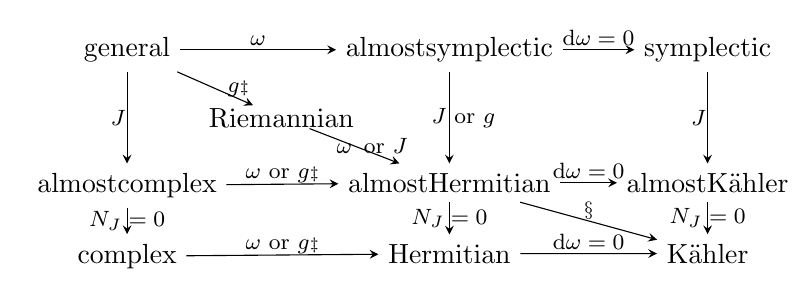
\begin{tikzpicture}
  \matrix (m) [matrix of nodes,row sep=1em,column sep=1em,minimum width=2em] {
     general & & \stackanchor{almost}{symplectic} & & symplectic \\
     & \clap{Riemannian} & & & \\
     \stackanchor{almost}{complex} & & \stackanchor{almost}{Hermitian} & & \stackanchor{almost}{K\"ahler} \\
%     & & & & \\
     complex & & Hermitian & & K\"ahler\\};
  \path[-stealth]
    (m-1-1) edge node [above=-.5ex] {\footnotesize $\omega$} (m-1-3)
    (m-1-1) edge node [right=.1em] {\footnotesize $g$\tabfootsymb{1}} (m-2-2)
    (m-1-1) edge node [left=-.3em] {\footnotesize $J$} (m-3-1)
    (m-1-3) edge node [above=-.5ex] {\footnotesize $\dd{\omega}=0$} (m-1-5)
    (m-1-3) edge node [right=-1em] {\footnotesize $J$ or $g$} (m-3-3)
    (m-1-5) edge node [left=-.3em] {\footnotesize $J$} (m-3-5)
    (m-2-2) edge node [right=-1em] {\footnotesize $\omega$\, or $J$} (m-3-3)
    (m-3-1) edge node [above=-.7ex] {\footnotesize $\omega$ or $g$\tabfootsymb{1}} (m-3-3)
            edge node {\footnotesize $N_J=0$} (m-4-1)
    (m-3-3) edge node [above=-.5ex] {\footnotesize $\dd{\omega}=0$} (m-3-5)
            edge node {\footnotesize $N_J=0$} (m-4-3)
            edge node [above=-.7ex] {\tabfootsymb{2}} (m-4-5)
    (m-3-5) edge node {\footnotesize $N_J=0$} (m-4-5)
    (m-4-1) edge node [above=-.7ex] {\footnotesize $\omega$ or $g$\tabfootsymb{1}} (m-4-3)
    (m-4-3) edge node [above=-.5ex] {\footnotesize $\dd{\omega}=0$} (m-4-5)
    ;
  \pgfresetboundingbox
  \path [use as bounding box] (m-3-1.west |- m-1-3.north) rectangle (m-1-5.east |- m-4-3.south);
\end{tikzpicture}
\end{tab}
(Almost)\,quaternionic/quaternion\-Hermitian/quaternion\-K\"ahler and
(almost)\,hyper\-complex/hyper\-Hermitian/hyper\-K\"ahler manifolds are
defined by replacing~$J$ by a 3d~subbundle of $\End TX$ or by global
sections $J_1,J_2,J_3$ as in the table of $G$-structures.
% ref: math/0307118 classification of "Almost Hermitian Structures and Quaternionic Geometries" (Francisco Martín Cabrera and Andrew Swann)
% ref: math/0105206 useful definitions in "Hyper-Hermitian quaternionic Kähler manifolds" (Bogdan Alexandrov)

\noindent\tabfoot{1}
Since $\Lie{GL}(n,\RR)/\Lie{O}(n)$ is contractible, any manifold admits
(non-canonically) an $\Lie{O}(n)$-structure, namely a smooth choice of
which frames are orthonormal, \ie, a Riemannian metric~$g$.  Similarly
$\Lie{GL}(n/2,\CC)/\Lie{U}(n/2)$ is contractible so almost complex
manifolds admit almost Hermitian structures.

\noindent\tabfoot{2}
An almost Hermitian manifold is K\"ahler if (equivalently) its
$\Lie{U}(n/2)$-structure is $1$-integrable; $\dd{\omega}=0$ and $N_J=0$;
$\nabla\omega=0$; $\nabla J=0$; or the holonomy group is in $\Lie{U}(n/2)$.
Locally, $\omega=\I\del\delbar\rho$ for some real-valued K\"ahler
potentials~$\rho$, and $\omega$~is invariant under K\"ahler transformations
$\rho\to\rho+f(z)+\bar{f}(\bar{z})$.



\paragraph{The holonomy group} at $x\in X$ of a connection~$\nabla$ on a
bundle $E\to X$ is the group of symmetries of~$E_x$ arising from
parallel transport along closed curves based at~$x$.

For Riemannian manifolds~$X$ the holonomy group is defined as that of
the Levi-Civita connection on the tangent bundle.  It is a subgroup of
$\Lie{O}(n)$ \big(or $\Lie{SO}(n)$ for $X$~orientable\big) since
parallel transport preserves orthogonality ($\nabla g=0$).

If the holonomy group acts reducibly on the tangent space then~$X$ is
locally (globally if $X$~is geodesically complete) a product.  Simply
connected~$X$ that are locally neither products nor symmetric spaces (we
give a list later) can have the following special holonomy subgroups of
$\Lie{SO}(n)$
(\href{https://ncatlab.org/nlab/show/Berger\%27s+theorem}{Berger's
  theorem})
\begin{tab}{lll}
  Holonomy & Manifold type & $\dim_{\RR}$\\
  \midrule
  % $\Lie{SO}(n)$ & orientable & $n$ \\
  $\Lie{U}(m)$ & K\"ahler & $2m$ \\
  $\Lie{SU}(m)$ & Calabi--Yau CY$_m$ & $2m$ \\
  \midrule
  $\bigl(\Lie{USp}(2k)\times\Lie{USp}(2)\bigr)/\cyclic{2}$ & quaternionic K\"ahler & $4k$ \\
  $\Lie{USp}(2k)$ & hyperK\"ahler & $4k$ \\
  \midrule
  $\Lie{Spin}(7)$ & $\Lie{Spin}(7)$ manifold & $8$ \\
  $\Lie{G}_2$ & $\Lie{G}_2$ manifold & $7$ \\
\end{tab}
% todo: more at https://en.wikipedia.org/wiki/Holonomy
% todo: perhaps http://projecteuclid.org/euclid.jdg/1090351387 interesting?
%
Note that $\Lie{U}(m)\supset\Lie{SU}(m)\supset\Lie{USp}(m)$ implies that
all hyperK\"ahler manifolds are Calabi--Yau and thus K\"ahler.
In general, quaternionic-K\"ahler manifolds are not K\"ahler.

% todo:
% A $\Lie{G}_2$-manifold is a $7$-dimensional manifold with a
% $1$-integrable $\Lie{G}_2\to\Lie{GL}(7)$ structure namely the
% corresponding definite 3-form $\omega$ should be covariantly constant
% with respect to the induced Riemannian metric (due to
% $\Lie{G}_2\subset \Lie{SO}(7)$.  Equivalently it is a Riemannian $7$-manifold
% with holonomy group~$\subseteq\Lie{G}_2$.

A \href{http://en.wikipedia.org/wiki/Calabi-Yau_manifold}{Calabi--Yau
  manifold} is a K\"ahler manifold such that (equivalently) some
K\"ahler metric has global holonomy group in $\Lie{SU}(m)$; the
structure group can be reduced to $\Lie{SU}(m)$; or the holomorphic
canonical bundle is trivial \ie, there exists a nowhere vanishing
holomorphic top-form.  A weaker set of equivalent conditions

\todo{here}

For simply connected manifolds, the conditions above are equivalent to
the following (always equivalent) conditions on~$X$: some K\"ahler
metric has local holonomy group in $\Lie{SU}(m)$; some K\"ahler metric
has vanishing Ricci curvature; the first real Chern class vanishes; a
positive power of the holomorphic canonical bundle is trivial; $X$~has a
finite cover with trivial holomorphic canonical bundle; $X$~has a finite
cover equal to the product of a torus and a simply connected manifold
with trivial holomorphic canonical bundle.

% todo: every Kähler manifold is spin (or at least spinc)

% todo: every hyperKähler manifold is Ricci-flat

% todo: every hyperKähler manifold is Calabi--Yau

% todo: ``Calabi proved a partial converse which says that a compact holomorphically symplectic Kähler manifold admits a unique hyper-Kähler metric with respect to any of its Kähler forms.'' (Mathworld)

% todo: more on http://mathworld.wolfram.com/Hyper-KaehlerManifold.html

% todo: more on Laplacians on Kähler manifolds at Wikipedia

% todo: HyperK\"ahler manifolds admit holomorphic symplectic forms (i.e. non-degenerate closed holomorphic $2$-form) $\omega_2+\I\omega_3$

% todo: Kodaira's classification of complex surfaces

% todo: complex submanifold of a Kähler manifold is Kähler, in particular projective algebraic varieties and Stein manifolds

% todo: Einstein manifold R=λg (but is λ constant?)

% todo: Kähler--Einstein manifold

% todo: self-dual Einstein manifolds

% Every quaternionic-K\"ahler manifold is locally almost hypercomplex

% Every quaternionic-K\"ahler manifold is Einstein

% A quaternionic-K\"ahler with zero scalar curvature is locally hyper-K\"ahler

% Compact hyperHermitian $4$-manifolds are conformal to tori, Hopf or K3. [ DOI: 10.2307/2046051 , Stable URL: http://www.jstor.org/stable/2046051 ]

\paragraph{Spin structures} \todo{see\quad \url{http://mathoverflow.net/questions/220502/}}

\paragraph{Symmetric spaces} \todo{list missing}

% todo: symmetric spaces? https://en.wikipedia.org/wiki/Symmetric_space

\paragraph{K3 surfaces} are the only CY$_2$: they have holonomy
$\Lie{SU}(2)$.

\paragraph{Yau's theorem.}  Fix a complex structure on a compact complex
manifold~$X$ of $\dim_{\CC}X>1$ and vanishing real first Chern class.
Any real class $H^{1,1}(X,\CC)$ of positive norm contains a unique
K\"ahler form whose metric is Ricci flat.

(from Wikipedia on Calabi conjecture: ``The Calabi conjecture states that a compact Kähler manifold has a unique Kähler metric in the same class whose Ricci form is any given 2-form representing the first Chern class.'')

% \subsection{Misc properties of manifolds}

% todo \paragraph{Rokhlin's theorem}

\section{Dualities}

\subsection{String theory dualities}

In this table ``type~IIA'' \etc{} refer to string theories not supergravities
\begin{tab}{l@{ $\Leftrightarrow$ }l}
  F-theory on K3 & $\Lie{E}_8\times\Lie{E}_8$ heterotic on~$T^2$ \\
  M-theory on K3 & heterotic or type~I on~$T^3$ \\
  Type~IIA on K3 & heterotic or type~I on~$T^4$ \\
  M-theory on $\Lie{G}_2$-manifolds\footnote{Apply K3 duality fiber-wise.} & heterotic or type~I on CY$_3$\\
  M-theory on K3\footnote{Apparently there is also a similar F-theory/heterotic duality.} & type~IIA on $T^3/\cyclic{2}$\\
\end{tab}

\section{Misc}

\subsection{Physics of gauge theories}

\paragraph{Phases characterized by potential} $V(R)$ between quarks (up to a constant):
Coulomb phase $1/R$,
free electric $1/\bigl(R\log(R\Lambda)\bigr)$,
free magnetic $\log(R\Lambda)/R$,
Higgs (constant),
confining $\sigma R$.

\subsection{Homotopy groups \(\pi\sb n\)}

\paragraph{Basic properties.} $\pi_0(X,x)$ is the set of connected components.  $\pi_1(X,x)$ is the fundamental group.  For $k\geq 1$, $\pi_k(X,x)$ only depends on the connected component of~$x$.  $\pi_k(X\times Y,(x,y))=\pi_k(X,x)\times\pi_k(Y,y)$.

\paragraph{Quotient.}  If $\pi_0(X)=\pi_1(X)=0$ and $G\actson X$ then $\pi_1(X/G)=\pi_0(G)$ ($=G$ for $G$~discrete).

\paragraph{Long exact sequence for a fiber bundle} $F\hookrightarrow E\twoheadrightarrow B$: for base-points $b_0\in B$ and $e_0=f_0\in F=p^{-1}(b_0)\subset E$, $\cdots\to\pi_{i+1}(B)\to\pi_i(F)\to\pi_i(E)\to\pi_i(B)\to\cdots\to\pi_0(E)$ is exact, namely each image equals the next kernel (inverse image of the constant map).

\paragraph{Homotopy groups of spheres} are finite except $\pi_n(S^n)=\ZZ$ and $\pi_{4n-1}(S^{2n})=\ZZ\times\text{finite}$.  For $k<n$, $\pi_k(S^n)=0$, and $\pi_{n+k}(S^n)$ is independent of~$n$ for $n\geq k+2$.  All $\pi_k(S^0)=0$, $\pi_k(S^1)=0$ for $k\neq 1$, and $\pi_k(S^3)=\pi_k(S^2)$ for $k\neq 2$.
\begin{tab}{*9{>{$}c<{$}}}
  & \pi_1 & \pi_2 & \pi_3 & \pi_4 & \pi_5 & \pi_6 & \pi_7 & \pi_8 \\\midrule
  S^0 & 0 & 0 & 0 & 0 & 0 & 0 & 0 & 0 \\
  S^1 & \ZZ & 0 & 0 & 0 & 0 & 0 & 0 & 0 \\
  S^2 & 0 & \ZZ & \ZZ & \ZZ_2 & \ZZ_2 & \ZZ_{12} & \ZZ_2 & \ZZ_2 \\
  S^3 & 0 & 0 & \ZZ & \ZZ_2 & \ZZ_2 & \ZZ_{12} & \ZZ_2 & \ZZ_2 \\
  S^4 & 0 & 0 & 0 & \ZZ & \ZZ_2 & \ZZ_2 & \ZZ\times \ZZ_{12} & \ZZ_2^2 \\
  S^5 & 0 & 0 & 0 & 0 & \ZZ & \ZZ_2 & \ZZ_2 & \ZZ_{24} \\
\end{tab}
% data of the table found on Wikipedia page


\paragraph{Topological groups have abelian \(\pi\sb 1(G)\).}
% http://mathoverflow.net/questions/35868/fundamental-group-of-lie-groups
Proofs.  1.\@ The multiplication in~$G$ (point-wise) and concatenation of loops are two compatible group structures, hence (by Eckmann--Hilton theorem) coincide and are commutative.  2.\@ Explicitly, for $\alpha_1,\alpha_2\in\pi_1(G)$ loops, $(t_1,t_2)\mapsto\alpha_1(t_1)\alpha_2(t_2)\in G$ is a homotopy between $\alpha_1\star\alpha_2$ (concatenation) along bottom and right edges, $\alpha_1\cdot\alpha_2$ (point-wise multiplication) along the diagonal, and $\alpha_2\star\alpha_1$ along left and top edges.

\subsection{K\"ahler \(4\)-manifolds}
 % see 1206.1070 for detailed exposition

\paragraph{K3~surfaces} are (the only besides~$T^4$) compact complex
surfaces of trivial canonical bundle.  They have $h^{1,0}=0$ (in
contrast to~$T^4$ which has \todo{value}).  Their first Chern class
$c_1\in H^2(X,\ZZ)$ thus vanishes.  By Yau's theorem there exists a
Ricci flat metric, whose holonomy is then $\Lie{SU}(2)=\Lie{USp}(2)$ by
Berger's classification.
% todo: which Sp?
K3~surfaces are thus Calabi--Yau (CY$_2$) and hyperK\"ahler (hK$_4$).
Their moduli space is connected and they are all diffeomorphic.

\paragraph{Examples of K3~surfaces.} Quartic hypersurface in~$\PP^4$.
Kummer surface namely resolution of $T^4/\cyclic{2}$.

% todo: maybe move closer to Yau's theorem in "Types of manifolds"?
\paragraph{Non-simply connected} Ricci-flat K\"ahler manifolds may fail
to be CY$_n$ when the restricted holonomy group is $\Lie{SU}(n)$ but the
global holonomy group is disconnected.  For example an Enriques surface
K3$/\cyclic{2}$ has a non-trivial canonical bundle.

\paragraph{Gravitational instantons.}  Ricci-flat metrics on hk$_4$ have
self-dual curvature and are called gravitational instantons.
% todo: only type of grav inst?
Compact hK$_4$ are K3 and~$T^4$.  Non-compact hK$_4$ are asymptotically
locally Euclidean (ALE) spaces asymptotic to $\HH/\Gamma$ for a finite
subgroup $\Gamma<\Lie{USp}(2)$.  Many such ALE spaces are local resolutions of
orbifold singularities of K3~surfaces.

\paragraph{} \todo{Taub-NUT spaces, multi-Taub-NUT spaces,
  Eguchi--Hanson spaces, Gibbons--Hawking multicenter spaces.  Write
  metric.}  \todo{Non-explicitly: Atiyah--Hitchin space (moduli space of
  two $\Lie{SU}(2)$ 't~Hooft-Polyakov monopoles in~4d).}

\todo{The only compact CY$_2$ are $T^4$ and K3~surfaces.}

\todo{The only compact hypercomplex $4$-manifolds are $T^4$,
  K3~surfaces, and the Hopf surface ($(\HH\setminus 0)/(q^\ZZ)$ for a
  quaternion $\abs{q}>1$; it is diffeomorphic to $S^3\times S^1$).}

% todo: what is the (co)homology of $X\times Y$?

% todo: In\"on\"u--Wigner contraction (for Lie superalgebras too)

% todo: vortices, monopoles, instantons (Abrikosov--Nielsen--Olesen
% vortex, 't~Hooft--Polyakov monopole, \ldots{}).


\bigskip
\vfill
\setlength{\parindent}{0pt}

%\begin{itemize}
%\item Say that only abelian $R$-symmetries can mix with global symmetries along the RG-flow.
%\end{itemize}


[1] \href{http://arxiv.org/abs/hep-th/9910030}{Tools for supersymmetry} by Antoine Van Proeyen

[2] Various Wikipedia articles.

[3] Various ncatlab.org articles.

\end{document}

% Local Variables:
% TeX-PDF-mode: t
% End:
